\documentclass[10pt, a4paper, oneside]{article}
\usepackage[ngerman]{babel}

\usepackage{multirow}

\usepackage{blindtext}
\usepackage{titlesec}
\usepackage{amsmath}
\usepackage[hidelinks]{hyperref}
\usepackage{parskip}
\usepackage{graphicx}
\usepackage{longtable}
\usepackage[shortlabels]{enumitem}
\usepackage{multirow}
\usepackage{nccmath}
\usepackage{rotating}
\usepackage{makecell}
\usepackage{multicol}
\usepackage{capt-of}
\usepackage{csquotes}
\usepackage{amsfonts}
\usepackage{caption}

\captionsetup[table]{position=bottom}

\titleformat{\section}
    {\normalfont\Large\bfseries}{}{0pt}{}

\let\oldsection\section
\renewcommand{\section}{
  \renewcommand{\theequation}{\thesection.\arabic{equation}}
  \oldsection}
\let\oldsubsection\subsection
\renewcommand{\subsection}{
  \renewcommand{\theequation}{\thesubsection.\arabic{equation}}
  \oldsubsection}

\makeatletter
\renewcommand{\maketitle}{
    \bgroup
    \centering
    \par\LARGE\@title  \\[20pt]
    \par\large\@author \\[10pt]
    \par\large\@date
    \par
    \egroup
}
\makeatother


\title{Wahrscheinlichkeitstheorie und Statistik\\[5pt]\Large L{\"o}sungen zu den Aufgaben 1, 5, 8 und 12}
\author{Volodymyr But}
\date{WS24/25, FHS Trier}

% - - - - - - - - - - - - - - - - - - - - - - - - - - - - - - - - - - - - - - %

\begin{document}

\maketitle
\vspace{25px}

\section{Aufgabe 1}

Stellen Sie sich vor, Sie sind Teil eines Forschungsteams, das eine Studie
"uber das Essverhalten in Großst"adten durchf"uhrt. Ihre Untersuchungseinheiten
sind Einwohner einer Großstadt. F"ur jede Untersuchungseinheit werden folgende
Merkmale erfasst.

\begin{enumerate}[-]
    \item Alter (in Jahren)
    \item Berufsgruppe (z.B Lehrer, Ingenieur, Student, usw.)
    \item Monatliches Einkommen (in Euro)
    \item Durchschnittliche Ausgaben f"ur Lebensmittel pro Woche (in Euro)
    \item Bevorzugte Art von Restaurant
    \item H"aufigkeit des Restaurantbesuchs pro Monat
    \item Bewertung der eigenen Kochf"ahigkeiten (auf eine Skala von 1 bis 5,
        wobei 1 sehr schlecht und 5 ausgezeichnet bedeutet)
\end{enumerate}

Klassifizieren Sie jedes dieser Merkmale als quantitativ oder qualitativ.
Unterteilen Sie weiter die qualitativen Merkmale in nominale und ordinale
Merkmale.

\textbf{L"osung}.

\bgroup
\def\arraystretch{1.5}
\begin{table}[h]
    \centering
    \begin{tabular}{p{0.33\linewidth}|p{0.33\linewidth}|p{0.33\linewidth}}
        \hfil\multirow{2}{*}{\centering quantitativ} & \multicolumn{2}{c}{qualitativ} \\
        \cline{2-3}
        & \hfil nominale & \hfil ordinale \\ \hline
        Alter & Berufsgruppe & Bevorzugte Art von Restaurant \\ \cline{1-1} \cline{3-3}
        Monatliches Einkommen & & Bewertung der Kochf"ahigkeiten \\ \cline{1-1}
        Durchschnittliche Ausgaben pro Woche & & \\ \cline{1-1}
        H"aufigkeit des Restaurantbesuchs pro Monat & &
    \end{tabular}
\end{table}
\egroup

\section{Aufgabe 5}

Betrachten Sie die Studienfachwahl von 200 Studienanf"angern an einer
Hochschule. Die Verteilung der Studienanf"anger auf die verschiedenen F"acher
ist wie folgt:

\begin{table}[h]
    \centering
    \begin{tabular}{l|c}
        \multicolumn{1}{l}{Studienfach} & \multicolumn{1}{c}{Anzahl der Studierenden} \\ \hline
        Informatik & 45 \\
        Architektur & 30 \\
        Wirtschaft & 25 \\
        Maschinenbau & 35 \\
        Elektrotechnik & 20 \\
        Lebensmitteltechnik & 25 \\
        Sonstige & 20
    \end{tabular}
\end{table}

\begin{enumerate}[1.]
    \item Bestimmen Sie die relativen H"aufigkeiten f"ur jedes Studienfach und
        berechnen Sie diese.

        \textbf{L"osung}.
        \begin{enumerate}[i)]
            \item $r_{\text{Informatik}} = \dfrac{45}{200} = 0,225$
            \item $r_{\text{Architektur}} = \dfrac{30}{200} = 0,15$
            \item $r_{\text{Wirtschaft}} = \dfrac{25}{200} = 0,125$
            \item $r_{\text{Maschinenbau}} = \dfrac{35}{200} = 0,175$
            \item $r_{\text{Elektrotechnik}} = \dfrac{20}{200} = 0,1$
            \item $r_{\text{Lebensmitteltechnik}} = \dfrac{25}{200} = 0,125$
            \item $r_{\text{Sonstige}} = \dfrac{20}{200} = 0,1$
        \end{enumerate}
    \vspace{10pt}
    \item Erstellen Sie ein Balkendiagramm, das die relativen H"aufigkeiten der
        Studienf"acher visualisiert.

        \textbf{L"osung}. Siehe Abbildung 1.

    \item Erstellen Sie ein Kreisdiagramm, das die gleichen Daten darstellt.

        \textbf{L"osung}. Siehe Abbildung 2.

    \item Diskutieren Sie, welches Diagramm geeigneter ist, um die Verteilung
        der Studienfachwahl darzustellen und warum.

        \textbf{Antwort}. Bei quantitativen Daten stellt das Balkendiagramm die
        Häufigkeit der Werte klarer dar als das Kreisdiagramm, weil es die
        einzelnen Werte entlang einer Achse sichtbar macht und Unterschiede in
        der Höhe der Balken auf einen Blick erkennbar sind.

    \pagebreak
    \begin{figure}[h]
        \centering
        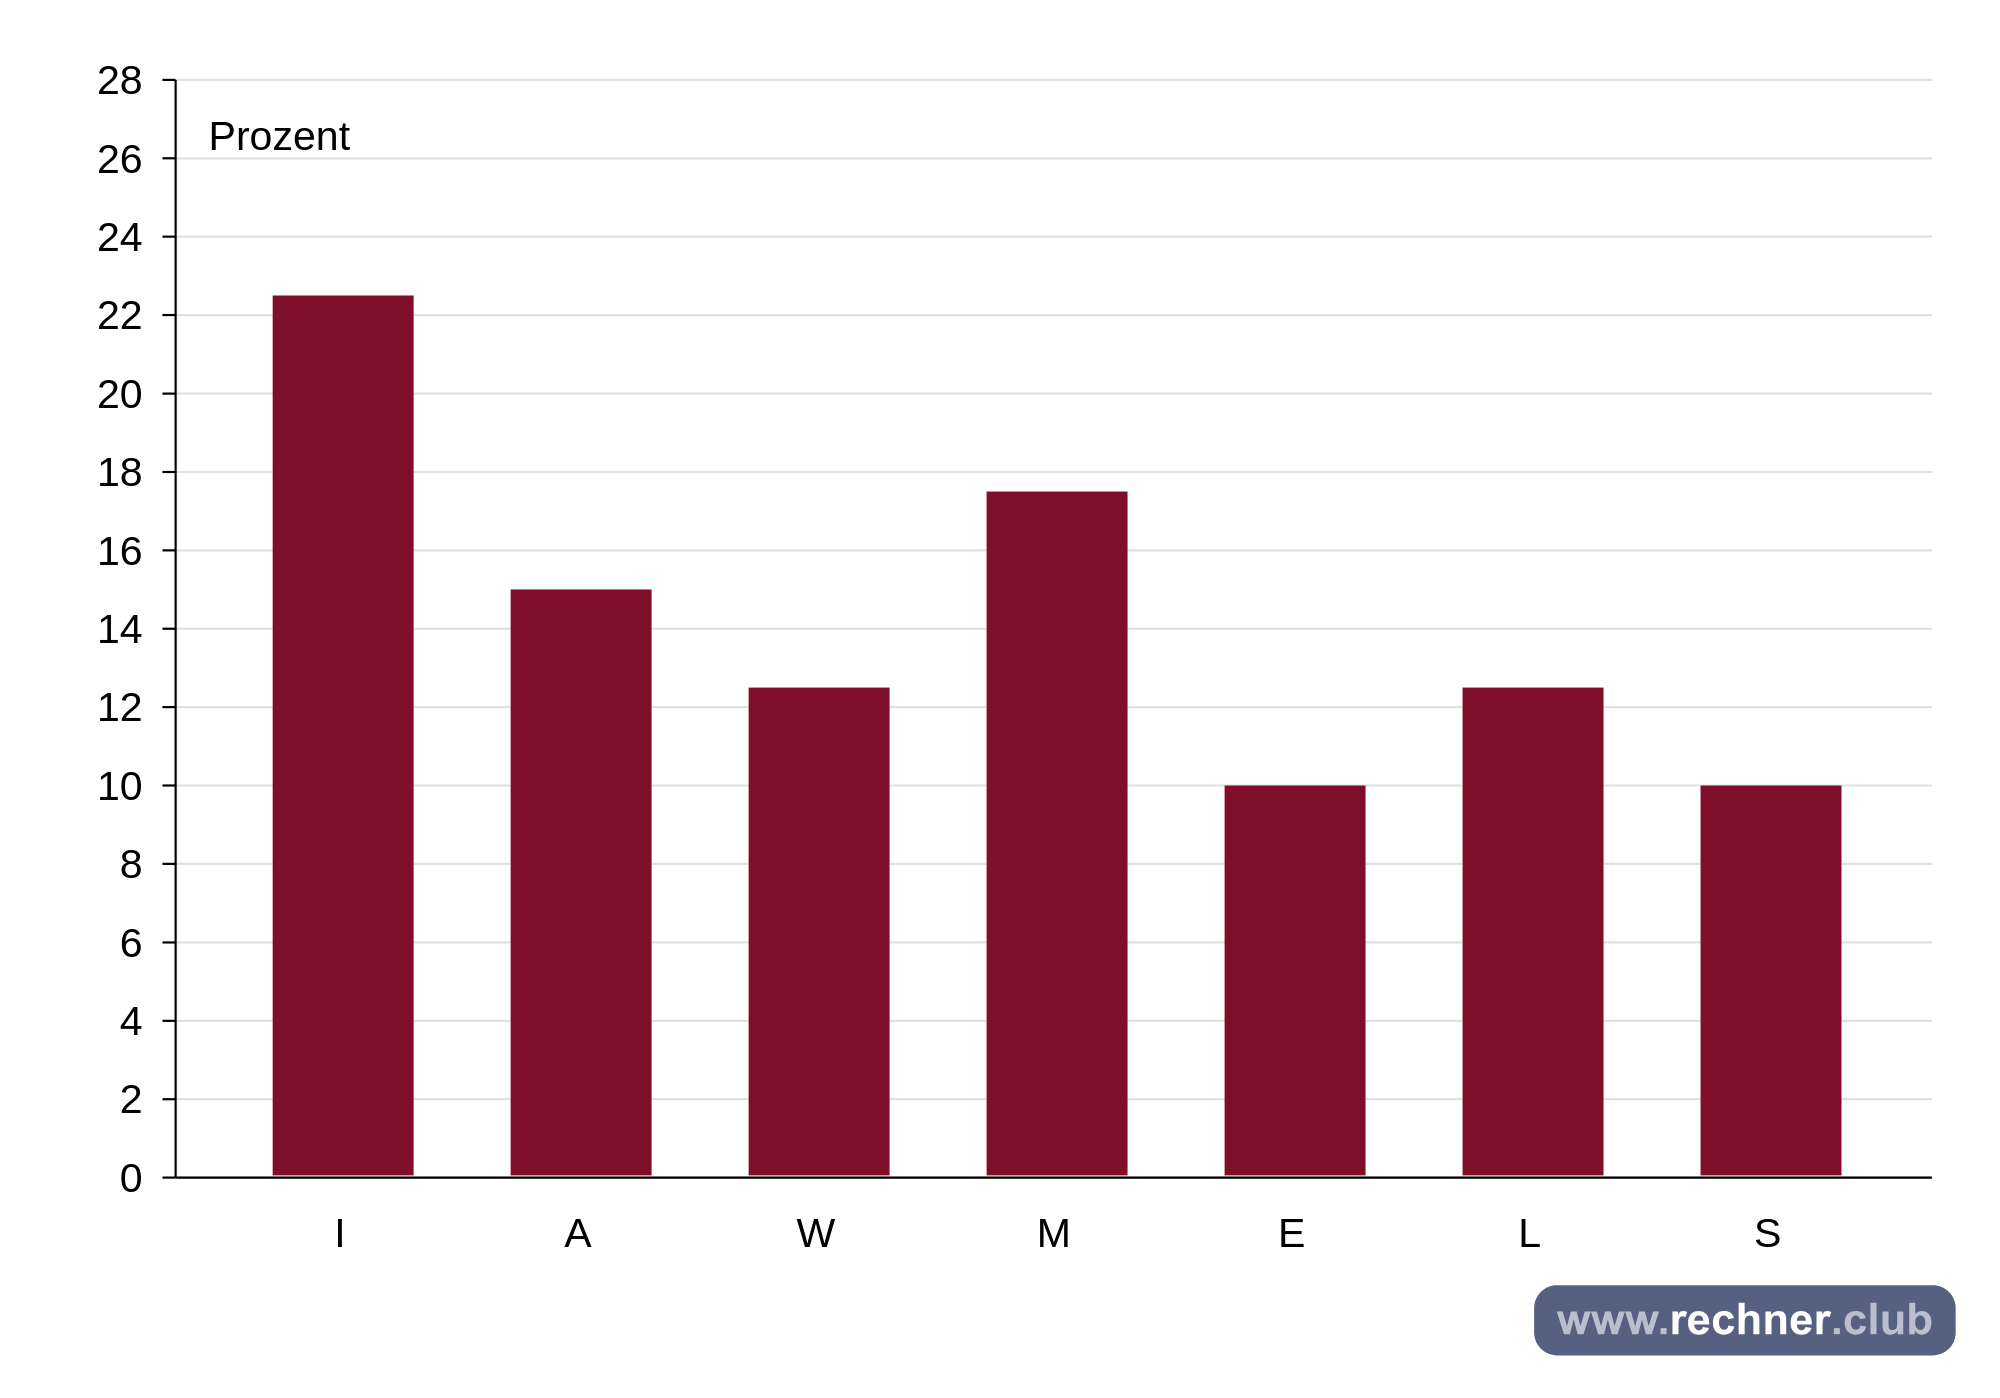
\includegraphics[width=0.8\textwidth]{./assets/saeulendiagramm-01.png}
        \caption{H"aufigkeit der Studienf"acher (Balkendiagramm)}
    \end{figure}

    \begin{figure}[!h]
        \centering
        \includegraphics[width=1\textwidth]{./assets/Kreisdiagramm-01.png}
        \caption{H"aufigkeit der Studienf"acher (Kreisdiagramm)}
    \end{figure}
    \pagebreak

\end{enumerate}

\section{Aufgabe 8}

In einer Studie zur Schlafdauer wurden folgende Schlafstunden pro Nacht von 40
Personen aufgezeichnet: (Es wird hier der Punkt zur Darstellung von Dezimal-
zahlen verwendet)

\begin{align*}
       8, 7, 6, 7.5, 9, 6.5, 7, 8.5, 6, 7&,\\
     7.5, 8, 5.5, 9, 7, 6.5, 7, 8, 9.5, 6&,\\
     7, 8.5, 6, 7.5, 8, 5.5, 7, 9, 6.5, 8&,\\
     7, 6, 8.5, 7.5, 9, 6.5, 8, 7, 9.5, 6&
\end{align*}

Konstruieren Sie ein Histogramm, um die Verteilung der Schlafdauer zu
visualisieren. Legen Sie die Intervalle so fest, dass sie die Verteilung der
Daten sinnvoll abbilden.

\textbf{L"osung}.

\begin{figure}[h]
    \centering
    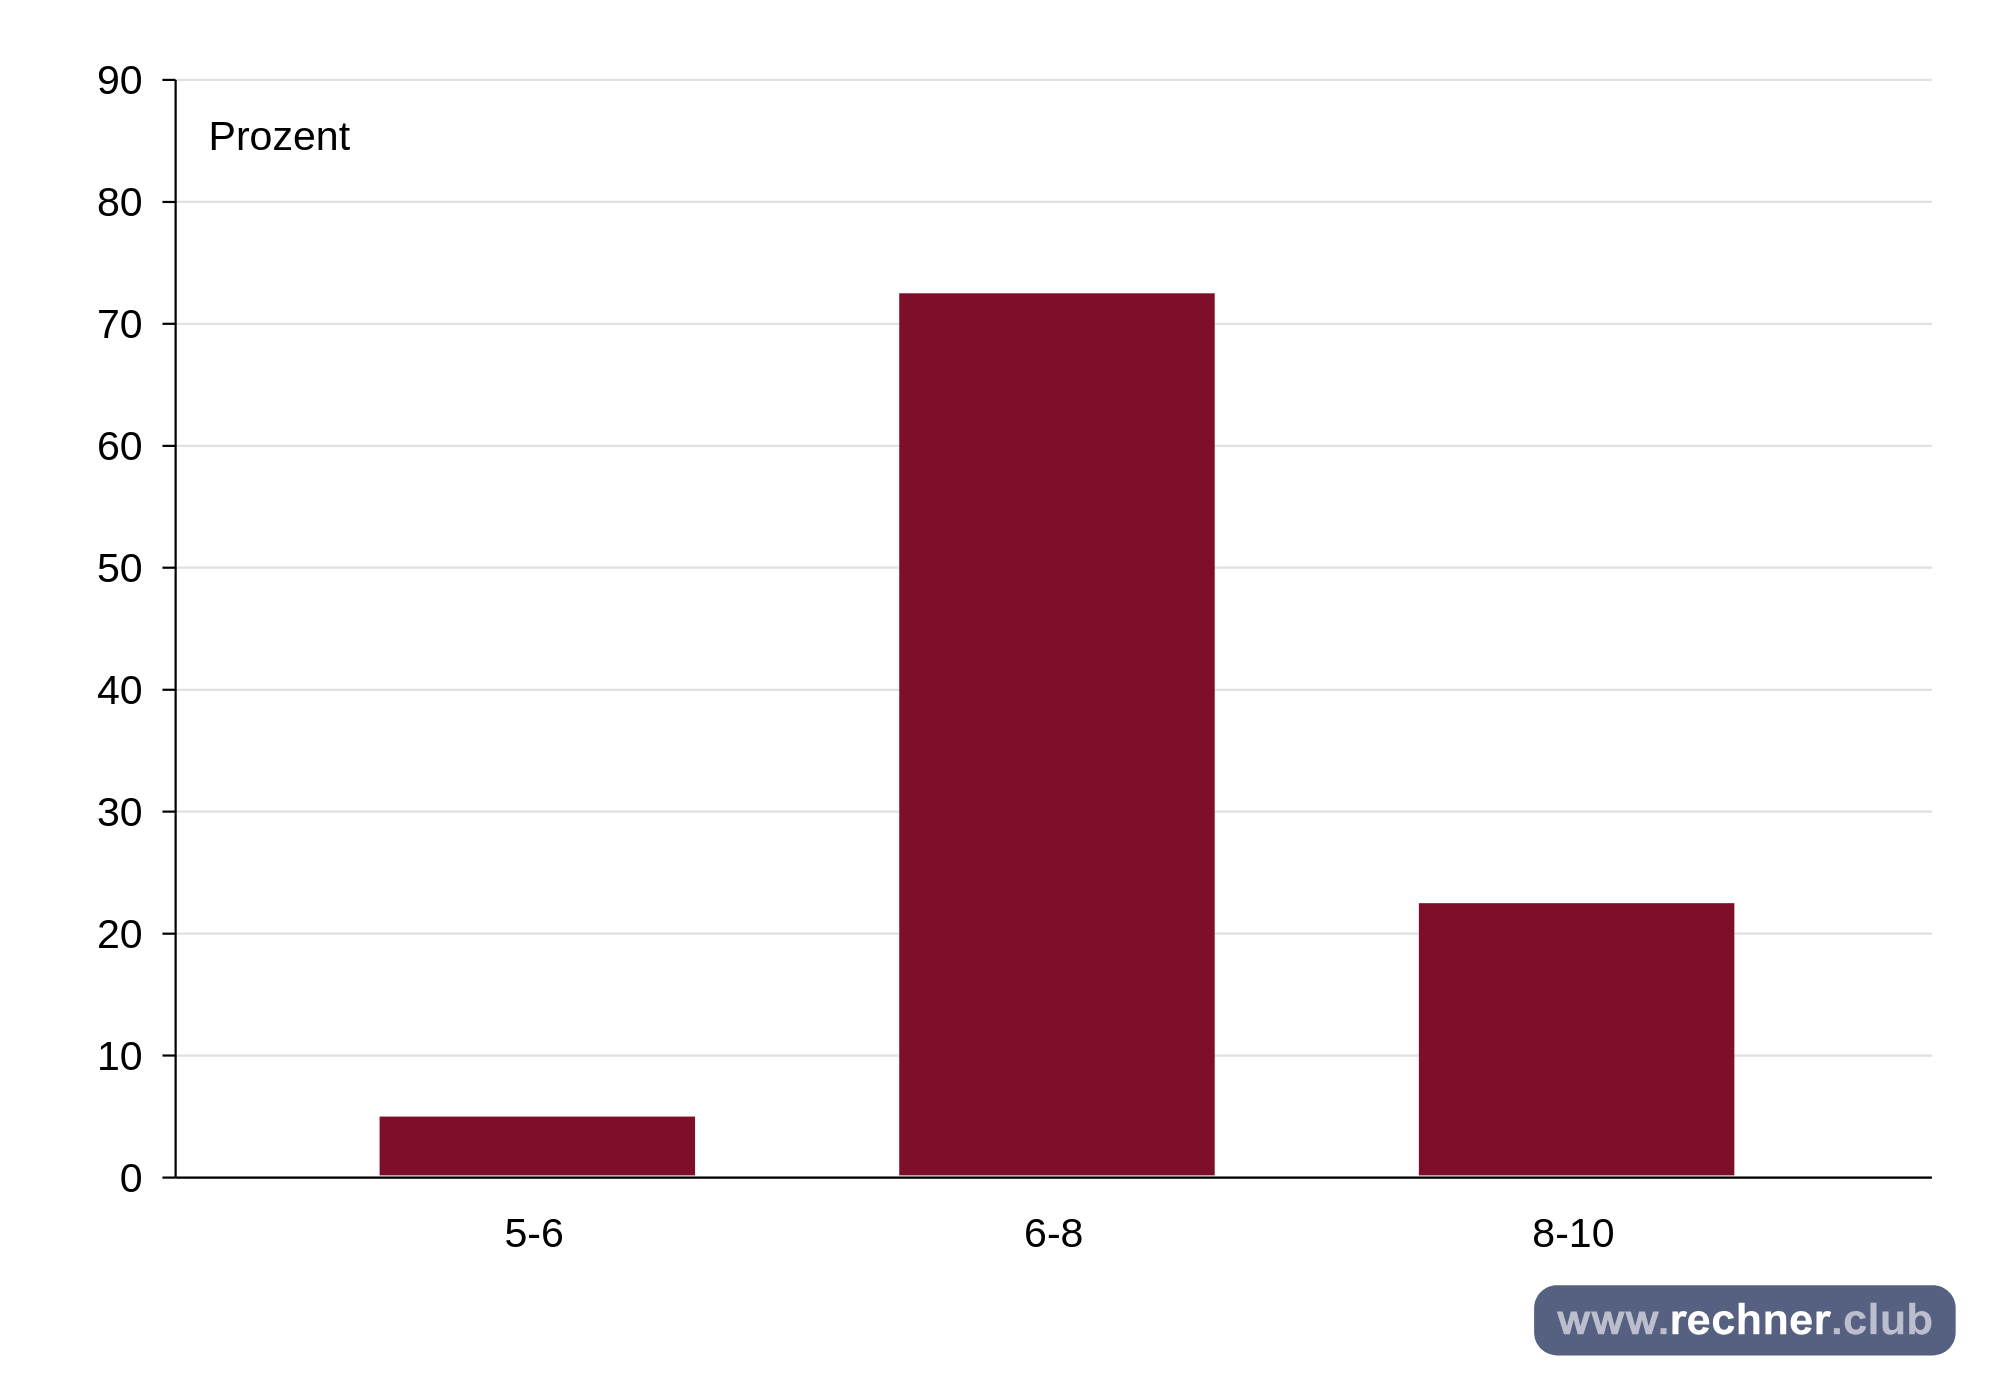
\includegraphics[width=1\textwidth]{./assets/saeulendiagramm-02.png}
    \caption{Verteilung der Schlafdauer}
\end{figure}

\pagebreak
\section{Aufgabe 12}

Ein mittelgroßes Unternehmen hat die folgenden monatlichen Gehaltsdaten (in
Tausend Euro) von 30 Mitarbeitern registriert:

\begin{align*}
        55, 60, 45, 40, 42, 48, 52, 50, 46, 44&,\\
        58, 60, 43, 41, 42, 57, 55, 46, 50, 40&,\\
    42, 45, 60, 55, 58, 57, 300, 290, 310, 320&
\end{align*}

Die letzten vier Werte stellen die Geh"alter der Top-Manager dar und sind
deutlich h"oher als die der "ubrigen Mitarbeiter.

\begin{enumerate}[1.]
    \item Berechnen Sie das arithmetische Mittle der Geh"alter.
        
        $$\bar{x} = \dfrac{1}{n}\sum_{k=1}^nx_k = \dfrac{2511}{30} = 83.7$$

    \item Bestimmen Sie den Median der Geh"alter.

        $$\widetilde{x} = \dfrac{1}{2}(x_{n/2} + x_{n/2 + 1}) = \dfrac{1}{2}(50 + 50) = 50$$

    \item Ermitteln Sie das 0,25-Quantil und das 0,75-Quantil.

        $$Q_{0.25} = x_8 = 44$$
        $$Q_{0.75} = x_{22} = 58$$

    \item Berechnen Sie das 0,1-getrimmte Mittel, um den Einfluss der Ausreißer
        zu mindern.

        $$\bar{x_{\alpha}} = \dfrac{1}{24}\sum_{k = 4}^{27}x_k = \dfrac{1}{24} \cdot 1460 = 60.833$$

    \item Bestimmen Sie die empirische Varianz und die Standardabweichung.

        $$s^2 = \dfrac{1}{n - 1}\sum_{k=1}^n(x_k - \bar{x})^2 = 7592,61$$
        $$\sigma = \sqrt{s^2} = 87.14$$

    \item Berechnen Sie die Spannweite der Geh"alter.

        $$\max_{1 \leq j \leq n}x_j - \min_{1 \leq j \leq n}x_j = 320 - 40 = 280$$

\end{enumerate}

\end{document}
